\scanpage{43}
c) Soit $G$ un groupe d'un Topos, \uline{Topos classifiant} $B_G$. (Il ``classifie'' les torseurs sous $G$ -- mais

\margin{\deleted{\unsure{Topos} \unsure{étalé}}}

\deleted{\unsure{$B_G$}} d) \uline{Topos induit} $E_{/X}$ (on identifie \unsure{souvent} $E$ avec son objet final, $E_{/X}$ avec $X$ ... )

\margin{\uline{l'objet} \uline{hom} \uline{\unsure{endomorphismes|homomorphismes}} \unsure{de} catégorie \uline{triviale}}

3) Morphismes de topos : \uline{forment une catégorie.}

\[\begin{aligned}\underline{\mathrm{MorTop}}(X,Y)&\lhook\joinrel\xrightarrow[\mathrm{plfid}]{}\underline{\mathrm{Hom}}\ \underline{\mathrm{cat}}\,(X,Y)\\ f&\longmapsto f_*\end{aligned}\]

% slanted
\margin{$\bullet$ Attention sens des flèches}

La composition des morphismes est un \unsure{accouplement} \deleted{Morphisme} de catégories, i.e. associatif : les topos forment une ``2-catégorie'' (pas seulement une catégorie).

% slanted
\margin{Attention ne pas passer trop hâtivement aux classes d'isomorphie des topos.}

Notion d'équivalence \inserted{de topos} : $f:X\to Y$ est une équivalence ssi $\exists\,g:Y\to X$ t. q. $gf\simeq\mathrm{id}_{\deleted{\unsure{Y}}X}$, $fg\simeq\mathrm{id}_Y$. Ici, c'est la notion habituelle d'équivalence de catégorie. C'est la notion qui remplace la notion d'isomorphie (= homéomorphie) pour les espaces topologiques.

4) Exemples de morphismes de topos

a) Cas de $\operatorname{Top}(X)$ : déjà étudié : $\operatorname{Top}(X)$ dépend de $X$ de façon covariante. On les identifie. $(\mathrm{Esp\ sob})$ \deleted{\unsure{$\to$}} peut être transformé en 2-catégorie. On a un foncteur 2-fidèle de cette \unsure{dernière} dans la 2-catégorie $(\mathrm{Top})$

a') (Cas de $\operatorname{Top}(X,G)$. \inserted{$(X,G)$ variable} (il n'y a plus de pleine fidélité

b) [Morphismes de $E$ dans $\operatorname{Top}(X)$ : pareil que \deleted{\unsure{foncteur|foutes}} applications $\operatorname{Ouv}(X)\longrightarrow\underbrace{\text{Ss-objets de }e_E}_{\text{ouverts de }E}$, commutant aux sup quelc. et aux $\cap$ finies.]

\uline{Ex} Si $X$ est un \uline{doublet} \inserted{(on écrit $\underline D$)}

\figure{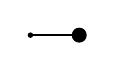
\begin{tikzpicture}[baseline=-.5ex]\draw[line width=.7pt] (0,0)--(.62,0);\fill (0,0) circle (.035);\fill (.62,0) circle (.095);\end{tikzpicture}}

($X=\{x,y\}$, \deleted{\unsure{$x\ne y$}} \deleted{$x\in\overline{\{y\}}$, $y\notin\{x\}$ $\{x\}$} $x$ fermé, $x\ne y$, $x\in\overline{\{y\}}$), alors la donnée de $E$ dans $\operatorname{Top}(X)$ équivaut à la donnée d'un ouvert de $E$ (\deleted{le Topos} \inserted{\unsure{l'objet|des} doublet} est topos classifiant pour l'espèce de structure : ss-objet de l'objet final)

\uline{NB} Tout espace top. de préordre se plonge dans un produit de doublets $\underline D^{I}$
% archive sheet number: 42
